\documentclass[11pt,a4paper]{article}

% Paquetes esenciales
\usepackage[utf8]{inputenc}
\usepackage[spanish]{babel}
\usepackage[margin=2.5cm]{geometry}
\usepackage{graphicx}
\usepackage{fancyhdr}
\usepackage{float}
\usepackage{amsmath}
\usepackage{booktabs}
\usepackage{hyperref}
\usepackage{xcolor}
\usepackage{caption}
\usepackage{subcaption}
\usepackage{titlesec}
\usepackage{multirow}
\renewcommand{\familydefault}{\sfdefault} % sans serif
\usepackage{helvet}

% Configuración de colores
\definecolor{azuloscuro}{RGB}{0,51,102}
\definecolor{grisclaro}{RGB}{240,240,240}
\definecolor{rojochurn}{RGB}{220,53,69}
\definecolor{verdeok}{RGB}{40,167,69}

% Configuración de hipervínculos
\hypersetup{
	colorlinks=true,
	linkcolor=azuloscuro,
	filecolor=magenta,      
	urlcolor=cyan,
	citecolor=azuloscuro,
}

% Configuración de títulos de sección
\titleformat{\section}
{\normalfont\Large\bfseries\color{azuloscuro}}{\thesection}{1em}{}
\titleformat{\subsection}
{\normalfont\large\bfseries\color{azuloscuro}}{\thesubsection}{1em}{}

% Configuración del encabezado y pie de página
\pagestyle{fancy}
\fancyhf{}

\fancyhead[L]{
\includegraphics[width=4cm]{logo1.png}}
\fancyhead[R]{
\includegraphics[width=4cm]{logo2.png}}

\fancyfoot[C]{\thepage}

\setlength{\headheight}{40pt}
\renewcommand{\headrulewidth}{0.9pt}
\renewcommand{\footrulewidth}{0.9pt}

% Portada sin encabezados
\fancypagestyle{plain}{
	\fancyhf{}
	\renewcommand{\headrulewidth}{0pt}
	\fancyfoot[C]{\thepage}
}

\begin{document}
	% ==================== PORTADA ====================
	\begin{titlepage}
		\centering
		\vspace*{1cm}
		
\includegraphics[width=2.5cm]{logo1.png}
		\hfill
		
\includegraphics[width=2.5cm]{logo2.png}		
		\vspace{2cm}
		
		{\Huge\bfseries\color{azuloscuro} Reporte Ejecutivo\par}
		\vspace{0.5cm}
		{\LARGE\textbf {Análisis Predictivo en Finanzas}\par}
		{\Large\textbf{MBD00011 - Magíster en Business Analytics}\par}
		
		
		
		\vfill
		
		{\large Daniel Avello - Felipe Valdivia - Roberto Sepúlveda\par}
		\vspace{0.3cm}
		{\large \today\par}
		
	\end{titlepage}


\section*{Resumen}

Este informe presenta los resultados del examen de Análisis Predictivo en Finanzas. El trabajo se organizó en tres bloques: simulaciones para estudiar regresión espuria, ejercicios de predictibilidad con \textit{commodity currencies}, y una aplicación de Box-Jenkins al GDP de Reino Unido.

En la Parte 1 se simularon series independientes bajo distintos niveles de persistencia. El punto central fue revisar qué ocurre cuando se estima una regresión entre variables que, por construcción, no tienen relación. En el caso estacionario los falsos rechazos fueron acotados, aunque no nulos; con alta persistencia aumentaron; y con caminatas aleatorias la inferencia usual rechazó en las diez regresiones. HAC redujo parte del problema, pero no lo eliminó cuando las series tenían raíz unitaria.

En la Parte 2 se evaluó la hipótesis de \textit{commodity currencies}. La evidencia dentro de muestra fue favorable en algunos casos, especialmente en aluminio y en especificaciones que incorporan el peso chileno. Sin embargo, al pasar a ejercicios fuera de muestra, los modelos con tipo de cambio no dominaron de forma sistemática al AR(1) ni a otros benchmarks simples. La evaluación económica mediante MDA, trading y portafolio tampoco mostró ganancias robustas. Por eso, la conclusión de esta parte es prudente: existe señal predictiva en casos específicos, pero no es estable ni fácil de explotar.

En la Parte 3 se aplicó la metodología Box-Jenkins. El GDP en nivel no rechazó raíz unitaria, mientras que la primera diferencia logarítmica sí presentó un comportamiento estacionario. Entre los modelos evaluados, el ARIMA(1,1,1) fue seleccionado por criterios de información, significancia de parámetros y diagnóstico de residuos.

La lectura general es que el análisis predictivo en finanzas exige más que encontrar coeficientes significativos. Antes de afirmar que un modelo predice, es necesario revisar estacionariedad, comparar contra benchmarks simples, evaluar fuera de muestra y verificar si la señal tiene alguna utilidad económica.

\newpage

\section{Introducción}

El examen se puede leer como una revisión aplicada de varios problemas que aparecen al trabajar con series financieras. No basta con estimar una regresión y mirar si el p-value es bajo. Antes de interpretar un resultado predictivo, hay que revisar si las series son estacionarias, si la relación se mantiene fuera de muestra y si el modelo supera a alternativas simples.

Bajo esa lógica, el informe se divide en tres partes. La primera usa simulaciones para mostrar cómo aparecen relaciones espurias cuando las series son persistentes o tienen raíz unitaria. La segunda evalúa la hipótesis de \textit{commodity currencies}, es decir, si algunos tipos de cambio contienen información útil para anticipar retornos de commodities. La tercera aplica la metodología Box-Jenkins para modelar el GDP de Reino Unido.

La idea no es forzar una conclusión optimista sobre predictibilidad. De hecho, varios resultados muestran que la evidencia se debilita cuando se exige validación fuera de muestra o valor económico. Por eso, el informe presenta tanto los resultados favorables como los casos donde los modelos no logran superar benchmarks simples.

\newpage
\section{Simulaciones y regresión espuria}

\subsection{Diseño del ejercicio}

Se generaron veinte procesos independientes en cada escenario. Los diez primeros se definieron como $Y_1,\dots,Y_{10}$ y los diez restantes como $X_1,\dots,X_{10}$. Luego se estimaron diez regresiones de la forma:

\begin{equation}
Y_{i,t}=c+kX_{i,t}+u_{i,t}, \quad i=1,\dots,10.
\end{equation}

Como las variables $X_i$ e $Y_i$ fueron generadas de forma independiente, el valor teórico del parámetro $k$ es cero. Por lo tanto, cualquier rechazo de $H_0:k=0$ corresponde a un falso rechazo. La comparación se hizo usando errores estándar usuales y errores estándar HAC.

Se revisaron tres escenarios: AR(1) estacionario con $b=0.6$, AR(1) altamente persistente con $b=0.97$ y caminata aleatoria con $b=1$. El interés no está solo en cada regresión individual, sino en cómo cambia la frecuencia de rechazos a medida que aumenta la persistencia.

\subsection{Resultados por escenario}

\begin{table}[H]
\centering
\caption{Resultados de regresión: AR(1) estacionario ($b=0.6$)}
\scriptsize
\begin{tabular}{lrrrrrr}
\toprule
Regresión & $\hat{k}$ & p-val usual & Sig. usual & p-val HAC & Sig. HAC & $R^2$ \\
\midrule
Y1 $\sim$ X1 & 0.0966 & 0.0030 & Sí & 0.0356 & Sí & 0.0088 \\
Y2 $\sim$ X2 & -0.0212 & 0.4925 & No & 0.6301 & No & 0.0005 \\
Y3 $\sim$ X3 & 0.0158 & 0.6445 & No & 0.7331 & No & 0.0002 \\
Y4 $\sim$ X4 & 0.0651 & 0.0403 & Sí & 0.1148 & No & 0.0042 \\
Y5 $\sim$ X5 & 0.0286 & 0.3711 & No & 0.5178 & No & 0.0008 \\
Y6 $\sim$ X6 & 0.0349 & 0.2996 & No & 0.4614 & No & 0.0011 \\
Y7 $\sim$ X7 & -0.0012 & 0.9699 & No & 0.9808 & No & 0.0000 \\
Y8 $\sim$ X8 & 0.0511 & 0.1027 & No & 0.2204 & No & 0.0027 \\
Y9 $\sim$ X9 & -0.0729 & 0.0285 & Sí & 0.1444 & No & 0.0048 \\
Y10 $\sim$ X10 & -0.1091 & 0.0007 & Sí & 0.0034 & Sí & 0.0115 \\
\bottomrule
\end{tabular}
\end{table}

En el caso estacionario, la inferencia usual rechaza 4 de 10 veces y HAC rechaza 2 de 10. La proporción usual es alta para un ejercicio al 10\%, pero debe leerse con cuidado porque el número de regresiones es pequeño. Lo importante es que los $R^2$ son muy bajos y no aparece una relación económica real entre las series.

\begin{table}[H]
\centering
\caption{Resultados de regresión: AR(1) altamente persistente ($b=0.97$)}
\scriptsize
\begin{tabular}{lrrrrrr}
\toprule
Regresión & $\hat{k}$ & p-val usual & Sig. usual & p-val HAC & Sig. HAC & $R^2$ \\
\midrule
Y1 $\sim$ X1 & -0.0956 & 0.0188 & Sí & 0.4146 & No & 0.0055 \\
Y2 $\sim$ X2 & -0.0028 & 0.9365 & No & 0.9810 & No & 0.0000 \\
Y3 $\sim$ X3 & -0.0654 & 0.1237 & No & 0.6442 & No & 0.0024 \\
Y4 $\sim$ X4 & 0.1037 & 0.0003 & Sí & 0.1858 & No & 0.0130 \\
Y5 $\sim$ X5 & -0.0526 & 0.1726 & No & 0.6325 & No & 0.0019 \\
Y6 $\sim$ X6 & 0.2289 & 0.0000 & Sí & 0.2220 & No & 0.0185 \\
Y7 $\sim$ X7 & 0.0294 & 0.3291 & No & 0.6882 & No & 0.0010 \\
Y8 $\sim$ X8 & -0.0091 & 0.7592 & No & 0.9179 & No & 0.0001 \\
Y9 $\sim$ X9 & -0.2760 & 0.0000 & Sí & 0.0003 & Sí & 0.0846 \\
Y10 $\sim$ X10 & -0.1381 & 0.0000 & Sí & 0.0607 & Sí & 0.0291 \\
\bottomrule
\end{tabular}
\end{table}

Al aumentar la persistencia a $b=0.97$, la inferencia usual rechaza 5 de 10 veces. HAC vuelve a dejar solo 2 rechazos. Este resultado muestra que parte de la significancia aparente se explica por la autocorrelación, aunque todavía no se está en el caso extremo de raíz unitaria.

\begin{table}[H]
\centering
\caption{Resultados de regresión: caminata aleatoria}
\scriptsize
\begin{tabular}{lrrrrrr}
\toprule
Regresión & $\hat{k}$ & p-val usual & Sig. usual & p-val HAC & Sig. HAC & $R^2$ \\
\midrule
Y1 $\sim$ X1 & -0.5218 & 0.0000 & Sí & 0.0001 & Sí & 0.1849 \\
Y2 $\sim$ X2 & -0.1082 & 0.0000 & Sí & 0.2221 & No & 0.0204 \\
Y3 $\sim$ X3 & 1.0138 & 0.0000 & Sí & 0.0000 & Sí & 0.5859 \\
Y4 $\sim$ X4 & 0.0713 & 0.0351 & Sí & 0.4228 & No & 0.0044 \\
Y5 $\sim$ X5 & 0.4358 & 0.0000 & Sí & 0.0000 & Sí & 0.2731 \\
Y6 $\sim$ X6 & 0.5454 & 0.0000 & Sí & 0.0012 & Sí & 0.2204 \\
Y7 $\sim$ X7 & 0.3302 & 0.0000 & Sí & 0.0000 & Sí & 0.4135 \\
Y8 $\sim$ X8 & 0.2598 & 0.0000 & Sí & 0.0009 & Sí & 0.1209 \\
Y9 $\sim$ X9 & 0.2076 & 0.0000 & Sí & 0.0118 & Sí & 0.0582 \\
Y10 $\sim$ X10 & -1.0607 & 0.0000 & Sí & 0.0000 & Sí & 0.7014 \\
\bottomrule
\end{tabular}
\end{table}

\begin{figure}[H]
	\centering		
	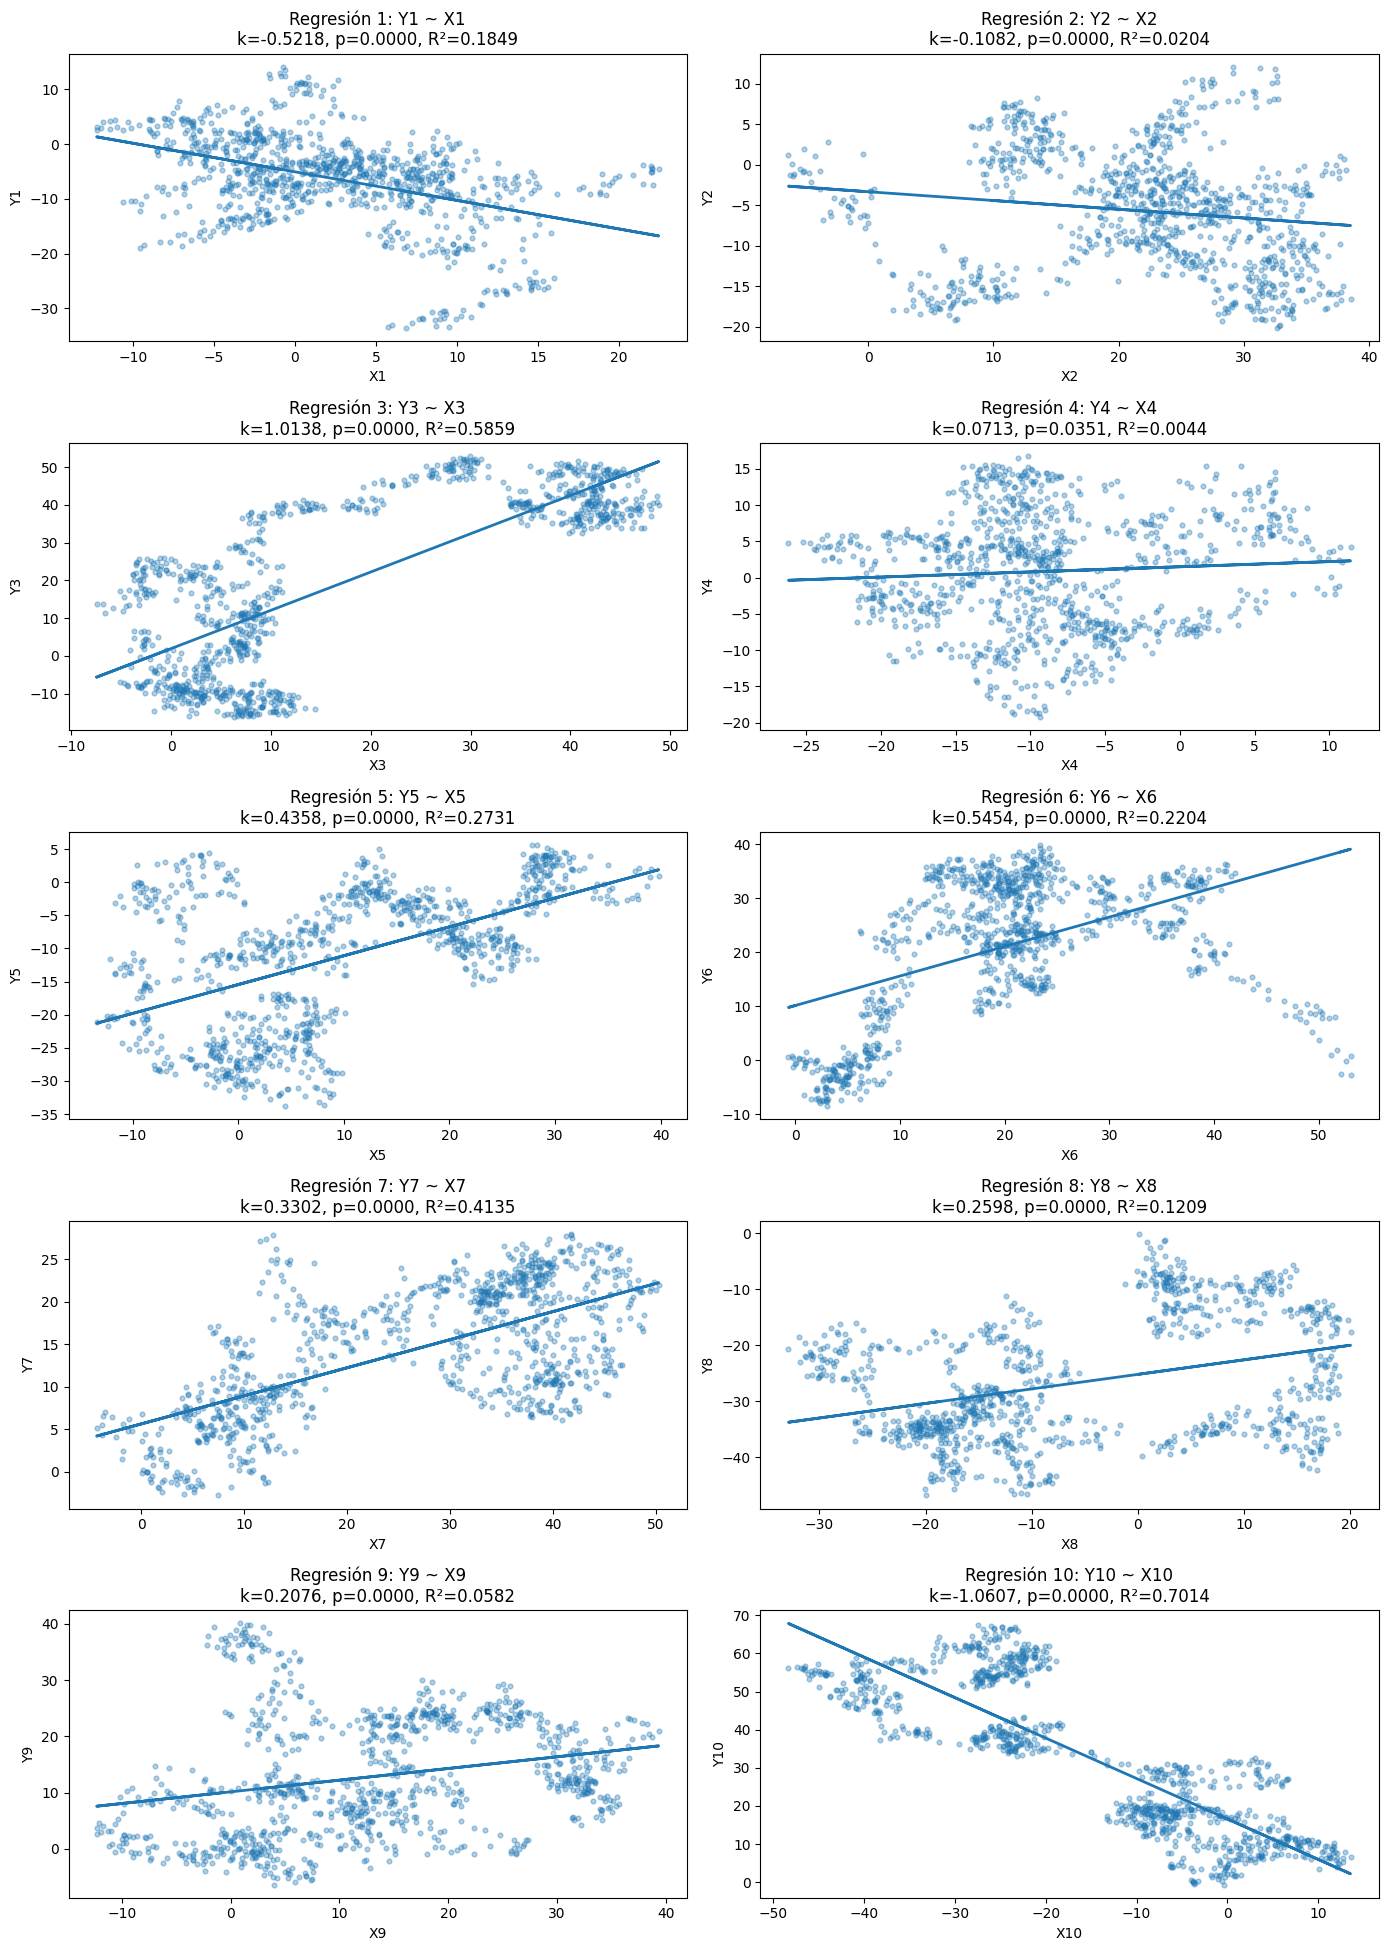
\includegraphics[width=0.9\textwidth]{Pregunta_iii_Random_Walk.png}		
	\caption{Regresiones entre caminatas aleatorias independientes}
	\label{fig:diagnostico_residuos}		
\end{figure}

El random walk es el caso donde el problema se ve con mayor claridad. La inferencia usual rechaza en el 100\% de las regresiones y HAC todavía rechaza en el 80\%. Además, varios $R^2$ son altos. Esto es engañoso, porque las series fueron generadas de forma independiente. La figura refuerza el punto: las trayectorias parecen moverse juntas o en direcciones opuestas, pero esa relación aparece por la persistencia de las series, no por un vínculo económico.

\begin{table}[H]
\centering
\caption{Resumen consolidado de simulaciones}
\begin{tabular}{lccccc}
\toprule
Escenario & $b$ & Nivel & \% usual & \% HAC & $R^2$ prom. \\
\midrule
AR(1) estacionario & 0.60 & 10\% & 40.0 & 20.0 & 0.0035 \\
AR(1) altamente persistente & 0.97 & 10\% & 50.0 & 20.0 & 0.0156 \\
Random walk & 1.00 & 5\% & 100.0 & 80.0 & 0.2583 \\
\bottomrule
\end{tabular}
\end{table}

\subsection{Interpretación de la Simulaciones y Regresión Espuria}

Si $k=0$ y se trabaja al 10\% de significancia, en condiciones estándar se esperaría rechazar cerca de 10\% de las veces. El ejercicio muestra que esa referencia pierde sentido cuando las series se vuelven muy persistentes. En particular, con caminatas aleatorias la inferencia tradicional deja de ser confiable, porque las distribuciones usuales de los estadísticos ya no son las que se están usando implícitamente en la prueba.

La lección práctica es simple: HAC ayuda, pero no arregla una regresión mal planteada con series no estacionarias. Antes de estimar relaciones predictivas en finanzas, conviene revisar raíz unitaria y transformar las series cuando corresponde.

\newpage
\section{Commodity currencies}

\subsection{Datos, transformaciones y estacionariedad}

La Parte 2 se trabajó con frecuencia mensual desde 1999M09. La base contiene tipos de cambio y commodities como aluminum, copper, lead, nickel, tin y LMEX. El enunciado menciona zinc, pero la base disponible no incluye esa columna; por eso el análisis se hizo con las series efectivamente presentes.

Primero se revisaron niveles, logaritmos y retornos. En niveles y logaritmos, las series muestran alta persistencia. En retornos, la persistencia baja de forma importante y las series se ven más compatibles con estacionariedad.

\begin{figure}[H]
	\centering		
	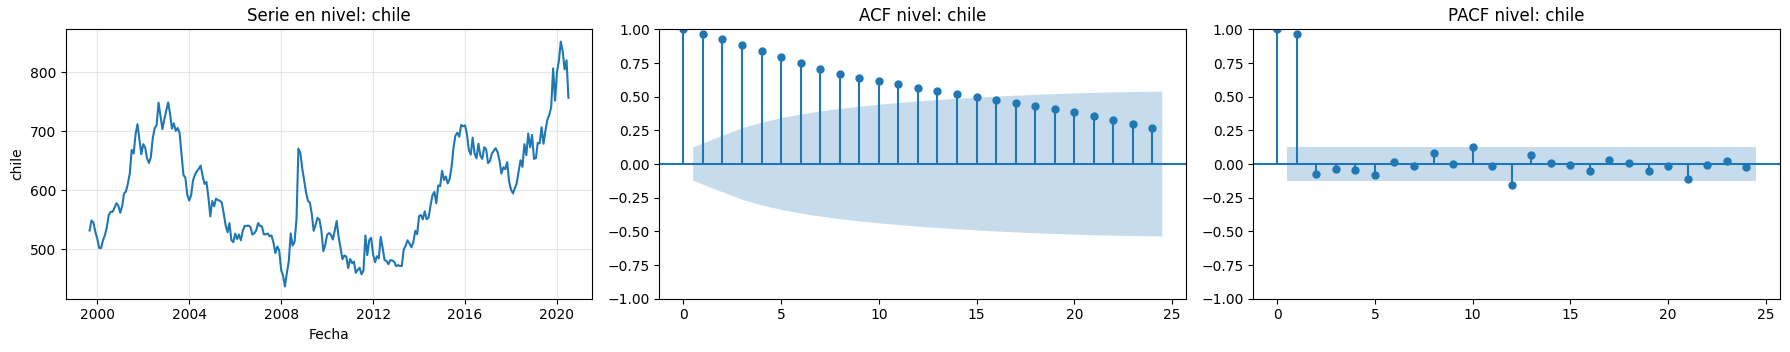
\includegraphics[width=0.9\textwidth]{grafico_1_Nivel_ACF_PACF_chile.png}		
	\caption{Tipo de cambio chileno en nivel: serie, ACF y PACF}
	\label{fig:diagnostico_residuos}		
\end{figure}



\begin{figure}[H]
\centering
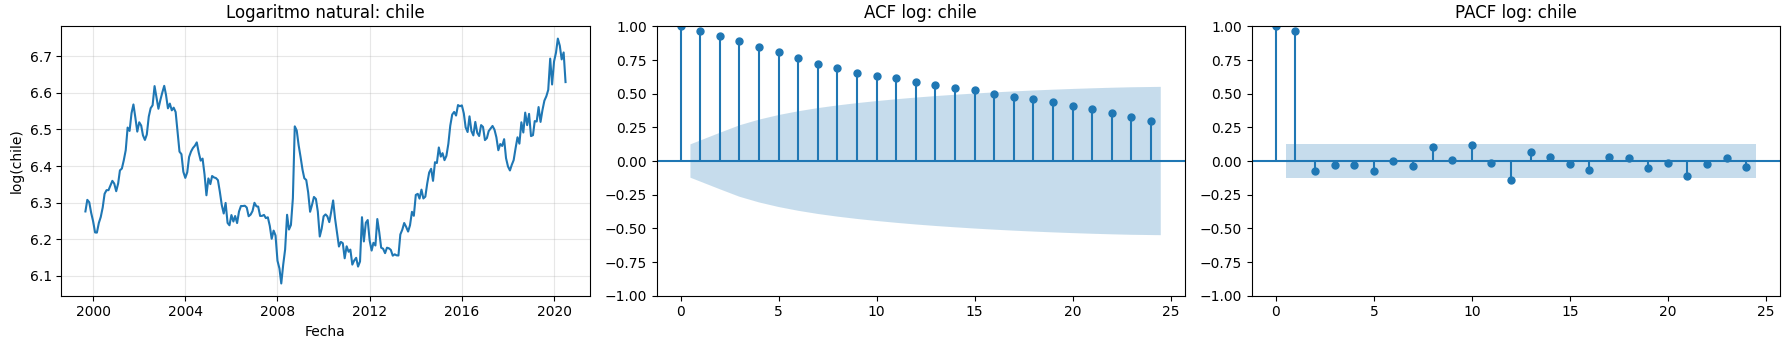
\includegraphics[width=0.9\textwidth]{grafico_2_Log_ACF_PACF_chile.png}
\caption{Tipo de cambio chileno en logaritmo: serie, ACF y PACF}
\end{figure}

\begin{figure}[H]
\centering
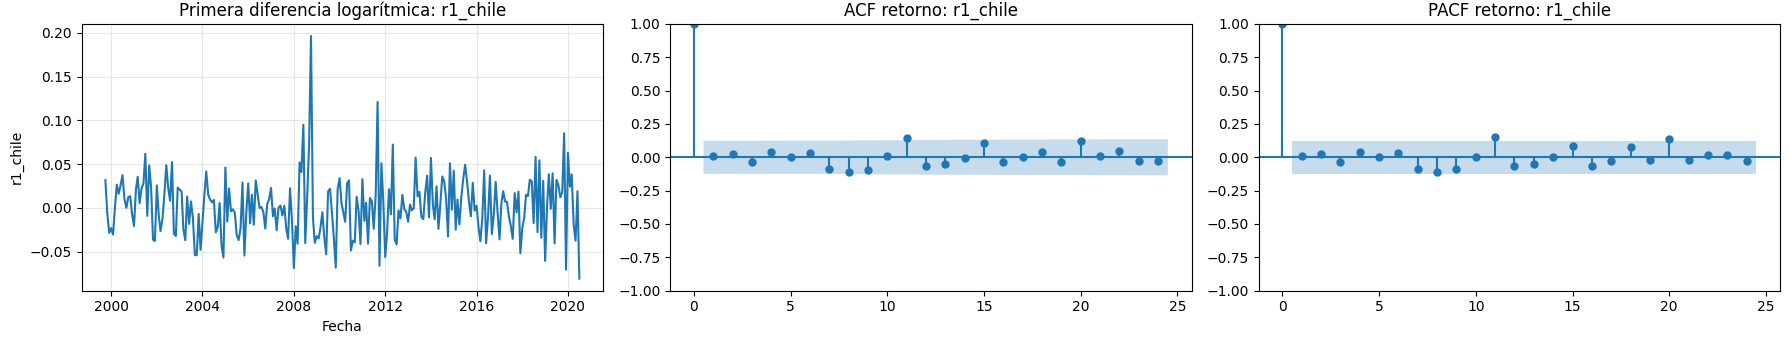
\includegraphics[width=0.9\textwidth]{grafico_3_Retornos_ACF_PACF_r1_chile.png}
\caption{Retorno logarítmico del tipo de cambio chileno: serie, ACF y PACF}
\end{figure}

El cambio entre las figuras es claro. En nivel y logaritmo, la ACF cae lentamente. En retorno, las autocorrelaciones quedan mucho más cerca de cero. Por eso las regresiones se realizaron con diferencias logarítmicas.

\begin{table}[H]
\centering
\caption{Resultados seleccionados del test ADF}
\begin{tabular}{llrrc}
\toprule
Serie & Transformación & ADF stat & p-value & Rechaza RU 5\% \\
\midrule
Chile & Nivel & -1.4589 & 0.5537 & No \\
Chile & Logaritmo & -1.4982 & 0.5344 & No \\
Chile & Retorno log & -15.4096 & 0.0000 & Sí \\
Australia & Nivel & -1.5188 & 0.5242 & No \\
Australia & Retorno log & -15.0744 & 0.0000 & Sí \\
Copper & Nivel & -2.0839 & 0.2510 & No \\
Copper & Retorno log & -8.6658 & 0.0000 & Sí \\
Aluminum & Nivel & -2.2837 & 0.1773 & No \\
\bottomrule
\end{tabular}
\end{table}

Los ADF confirman la lectura visual: precios y tipos de cambio en nivel no rechazan raíz unitaria, mientras que los retornos sí lo hacen. Esto es consistente con trabajar los modelos predictivos en retornos.

\subsection{Modelo CRR dentro de muestra}

La especificación de Chen, Rogoff y Rossi agrega un rezago del tipo de cambio a un AR(1) del retorno del commodity:

\begin{equation}
\Delta \log(C_t)=c+\rho\Delta \log(C_{t-1})+\beta\Delta \log(TC_{t-1})+\varepsilon_t.
\end{equation}

En los resultados seleccionados, la evidencia más clara aparece en aluminum. Para Chile, el coeficiente del tipo de cambio es -0.2883 y tiene p-value 0.0136. Para Australia, el coeficiente es -0.3199 y tiene p-value 0.0061. En copper y LMEX no se observa significancia al 5\%.

\begin{table}[H]
\centering
\caption{Resultados predictivos in-sample tipo CRR}
\scriptsize
\begin{tabular}{llrrrrrrr}
\toprule
Commodity & TC & $\rho$ AR & p-val $\rho$ & Sig. $\rho$ & $\beta_{TC}$ & p-val $\beta$ & Sig. $\beta$ & $\Delta R^2$ \\
\midrule
Copper & Chile & 0.1166 & 0.1106 & No & -0.2067 & 0.1962 & No & 0.0066 \\
Copper & Australia & 0.1190 & 0.1195 & No & -0.1643 & 0.2938 & No & 0.0044 \\
Aluminum & Chile & -0.0284 & 0.6750 & No & -0.2883 & 0.0136 & Sí & 0.0245 \\
Aluminum & Australia & -0.0650 & 0.3686 & No & -0.3199 & 0.0061 & Sí & 0.0302 \\
LMEX & Chile & 0.0835 & 0.2641 & No & -0.2114 & 0.1157 & No & 0.0098 \\
LMEX & Australia & 0.0716 & 0.3715 & No & -0.2041 & 0.1300 & No & 0.0091 \\
\bottomrule
\end{tabular}
\end{table}

La interpretación es acotada. No se observa que todos los tipos de cambio predigan todos los commodities. Más bien, la evidencia aparece en casos puntuales, especialmente aluminum.

\subsection{Errores HAC y cambio en la inferencia}

Al repetir el ejercicio con errores HAC, la conclusión principal se mantiene, aunque los p-values aumentan. Aluminum sigue siendo significativo tanto con Chile como con Australia, mientras que copper y LMEX no muestran evidencia robusta.

\begin{table}[H]
\centering
\caption{Resultados in-sample con errores HAC}
\scriptsize
\begin{tabular}{llrrrrrrr}
\toprule
Commodity & TC & $\rho$ AR & p-val $\rho$ & Sig. $\rho$ & $\beta_{TC}$ & p-val $\beta$ & Sig. $\beta$ & $\Delta R^2$ \\
\midrule
Copper & Chile & 0.1166 & 0.2201 & No & -0.2067 & 0.2177 & No & 0.0066 \\
Copper & Australia & 0.1190 & 0.2351 & No & -0.1643 & 0.3715 & No & 0.0044 \\
Aluminum & Chile & -0.0284 & 0.7568 & No & -0.2883 & 0.0342 & Sí & 0.0245 \\
Aluminum & Australia & -0.0650 & 0.5406 & No & -0.3199 & 0.0414 & Sí & 0.0302 \\
LMEX & Chile & 0.0835 & 0.3992 & No & -0.2114 & 0.1418 & No & 0.0098 \\
LMEX & Australia & 0.0716 & 0.5015 & No & -0.2041 & 0.2009 & No & 0.0091 \\
\bottomrule
\end{tabular}
\end{table}

Este contraste es útil porque muestra que la significancia no debe depender solo de errores estándar usuales. Si una relación se mantiene con HAC, al menos es más defendible dentro de muestra.

\subsection{Especificaciones Pincheira-Hardy}

La especificación Pincheira-Hardy incorpora dos rezagos del tipo de cambio:

\begin{equation}
\Delta \log(C_t)=c+\rho\Delta \log(C_{t-1})+\beta_1\Delta \log(TC_{t-1})+\beta_2\Delta \log(TC_{t-2})+\varepsilon_t.
\end{equation}

Para el peso chileno, el test conjunto $H_0:\beta_1=\beta_2=0$ entrega evidencia para tin, LMEX, lead, copper y aluminum. Nickel es el caso donde la evidencia es más débil. Esto sugiere que parte de la información predictiva puede estar distribuida en más de un rezago.

También se estimó una versión restringida usando la suma de los dos rezagos del tipo de cambio. Esa restricción reduce el número de parámetros. Para Chile, la pérdida de $R^2$ es baja en la mayoría de los commodities: tin, copper y aluminum caen alrededor de 0.001 a 0.002. La mayor caída aparece en lead. Por eso, la restricción parece razonable cuando se busca parsimonia, aunque no necesariamente domina en todos los casos.

\subsection{Evaluación fuera de muestra}

La evaluación fuera de muestra es más exigente que el ajuste in-sample. En lugar de usar toda la muestra para estimar, se separa una ventana de estimación y otra de evaluación. Luego se pronostica un paso adelante, actualizando los parámetros con ventanas recursivas y rodantes.

En el setup 30\%-70\%, el modelo PH con dos rezagos no supera al AR(1) para copper con Chile en las ventanas recursiva y rodante. En algunos casos, el zero forecast presenta menor ECM.

\begin{table}[H]
\centering
\caption{Ejemplos fuera de muestra: división 30\%-70\%}
\scriptsize
\begin{tabular}{lllrrrrc}
\toprule
Commodity & TC & Ventana & Modelo & ECM & $R^2_{OOS}$ & p-val DM & Mejor que AR(1) \\
\midrule
Copper & Chile & Recursive & PH dos rezagos & 0.0064 & -0.0077 & 0.7801 & No \\
Copper & Chile & Recursive & AR(1) & 0.0064 & 0.0000 & -- & -- \\
Copper & Chile & Recursive & Prom. histórico & 0.0064 & -0.0087 & 0.8717 & No \\
Copper & Chile & Recursive & Zero forecast & 0.0063 & 0.0066 & 0.8911 & Sí \\
Copper & Chile & Rolling & PH dos rezagos & 0.0065 & -0.0126 & 0.6512 & No \\
Copper & Chile & Rolling & AR(1) & 0.0065 & 0.0000 & -- & -- \\
Copper & Chile & Rolling & Zero forecast & 0.0063 & 0.0184 & 0.7578 & Sí \\
\bottomrule
\end{tabular}
\end{table}

En el setup 50\%-50\%, también aparecen benchmarks simples con buen desempeño. Para copper con Chile, el promedio histórico y el zero forecast superan al AR(1) y tienen diferencias significativas en algunos casos, mientras que PH no mejora al AR(1).

\begin{table}[H]
\centering
\caption{Ejemplos fuera de muestra: división 50\%-50\%}
\scriptsize
\begin{tabular}{lllrrrrc}
\toprule
Commodity & TC & Ventana & Modelo & ECM & $R^2_{OOS}$ & p-val DM & Mejor que AR(1) \\
\midrule
Copper & Chile & Recursive & PH dos rezagos & 0.0043 & -0.0238 & 0.5848 & No \\
Copper & Chile & Recursive & AR(1) & 0.0042 & 0.0000 & -- & -- \\
Copper & Chile & Recursive & Prom. histórico & 0.0037 & 0.1020 & 0.0466 & Sí \\
Copper & Chile & Recursive & Zero forecast & 0.0036 & 0.1287 & 0.0225 & Sí \\
Copper & Chile & Rolling & PH dos rezagos & 0.0044 & -0.0246 & 0.5696 & No \\
Copper & Chile & Rolling & Prom. histórico & 0.0038 & 0.1098 & 0.0358 & Sí \\
Copper & Chile & Rolling & Zero forecast & 0.0036 & 0.1498 & 0.0107 & Sí \\
\bottomrule
\end{tabular}
\end{table}

La diferencia entre in-sample y out-of-sample es una de las partes más importantes del ejercicio. Dentro de muestra se encuentran señales, pero fuera de muestra esas señales no dominan de manera estable. Esto puede deberse a inestabilidad de parámetros, sobreajuste o simplemente a que la señal predictiva es débil frente al ruido de los retornos financieros.

\subsection{MDA y estrategia de trading}

La Mean Directional Accuracy evalúa si el modelo acierta la dirección del retorno. En los casos reportados, la MDA queda cerca del 50\% o por debajo. Por ejemplo, el modelo PH con copper-Chile obtiene 0.4597 en ventana recursiva y 0.4677 en ventana rodante. Ninguno supera significativamente el benchmark de suerte pura.

\begin{table}[H]
\centering
\caption{Ejemplos de Mean Directional Accuracy}
\scriptsize
\begin{tabular}{llllrrc}
\toprule
Commodity & TC & Ventana & Modelo & MDA & p-value unilateral & Supera 50\% \\
\midrule
Copper & Chile & Recursive & PH dos rezagos & 0.4597 & 0.7957 & No \\
Copper & Chile & Recursive & AR(1) & 0.4194 & 0.9618 & No \\
Copper & Chile & Recursive & Prom. histórico & 0.5081 & 0.4222 & No \\
Copper & Chile & Rolling & PH dos rezagos & 0.4677 & 0.7570 & No \\
Copper & Chile & Rolling & AR(1) & 0.4597 & 0.8188 & No \\
Copper & Australia & Recursive & PH dos rezagos & 0.4194 & 0.9586 & No \\
\bottomrule
\end{tabular}
\end{table}

La estrategia de trading entrega una conclusión similar. Los retornos medios no son estadísticamente significativos en los modelos PH reportados. Por lo tanto, una mejora marginal en error de predicción no alcanza para construir una señal económica clara.

\begin{table}[H]
\centering
\caption{Ejemplos de estrategia de trading}
\scriptsize
\begin{tabular}{llllrrrc}
\toprule
Commodity & TC & Ventana & Modelo & Ret. medio & Ret. anual & p-value HAC & Significativo \\
\midrule
Copper & Chile & Recursive & PH dos rezagos & 0.0007 & 0.0088 & 0.8731 & No \\
Copper & Chile & Recursive & AR(1) & -0.0052 & -0.0622 & 0.2671 & No \\
Copper & Chile & Recursive & Prom. histórico & -0.0015 & -0.0183 & 0.7513 & No \\
Copper & Chile & Rolling & PH dos rezagos & 0.0011 & 0.0133 & 0.8137 & No \\
Copper & Chile & Rolling & AR(1) & -0.0042 & -0.0505 & 0.4175 & No \\
Copper & Australia & Recursive & PH dos rezagos & -0.0042 & -0.0505 & 0.3820 & No \\
\bottomrule
\end{tabular}
\end{table}

\subsection{Bonus 1: portafolio tipo Neely et al.}

El bonus de portafolio se incluyó para revisar si la señal predictiva mejora una decisión de inversión. Se usó una tasa libre de riesgo anual de 3\%, costos de transacción y dos niveles de aversión al riesgo ($\gamma=3$ y $\gamma=5$).

Los resultados no muestran una ventaja consistente. En varios casos el Sharpe es negativo y los excesos medios no son significativos. Para copper-Chile con PH dos rezagos y ventana recursiva, el retorno anualizado es 2.28\% con $\gamma=3$, pero el exceso medio no es significativo. Con $\gamma=5$, el retorno anualizado cae a 0.94\% y tampoco hay significancia.

\begin{table}[H]
\centering
\caption{Ejemplos de portafolio tipo Neely et al.}
\scriptsize
\begin{tabular}{llllrrrrr}
\toprule
Commodity & TC & Modelo & $\gamma$ & Ret. anual & Vol. anual & Sharpe & CER & p-value HAC \\
\midrule
Copper & Chile & PH dos rezagos & 3 & 0.0228 & 0.2171 & -0.0313 & -0.0479 & 0.9123 \\
Copper & Chile & PH dos rezagos & 5 & 0.0094 & 0.1820 & -0.1108 & -0.0734 & 0.7053 \\
Copper & Chile & AR(1) & 3 & -0.0628 & 0.1831 & -0.5043 & -0.1131 & 0.0799 \\
Copper & Chile & AR(1) & 5 & -0.0531 & 0.1371 & -0.6036 & -0.1001 & 0.0380 \\
Copper & Chile & Prom. histórico & 3 & -0.0125 & 0.1481 & -0.2846 & -0.0454 & 0.3155 \\
Copper & Chile & Zero forecast & 3 & 0.0296 & 0.0000 & -- & 0.0296 & -- \\
\bottomrule
\end{tabular}
\end{table}

La lectura práctica es que la señal predictiva no alcanza para construir una estrategia de portafolio claramente superior, sobre todo cuando se consideran volatilidad y costos.

\subsection{Bonus 2: paradoja del MSPE}

El segundo bonus revisa la paradoja del MSPE. Esta aparece cuando un modelo tiene peor error cuadrático medio que el benchmark, pero mayor correlación con la variable objetivo. En los resultados hay casos donde PH tiene peor ECM que AR(1), pero mayor correlación. Sin embargo, las diferencias de correlación no son significativas al 5\%.

\begin{table}[H]
\centering
\caption{Ejemplos de paradoja del MSPE}
\scriptsize
\begin{tabular}{llllrrrrc}
\toprule
Commodity & TC & Ventana & Modelo & ECM modelo & ECM AR(1) & $\Delta$ corr. & p-val boot & Sig. 5\% \\
\midrule
Copper & Chile & Recursive & PH dos rezagos & 0.0043 & 0.0042 & 0.0677 & 0.2953 & No \\
Copper & Chile & Rolling & PH dos rezagos & 0.0044 & 0.0043 & 0.0569 & 0.3724 & No \\
Copper & Australia & Recursive & PH dos rezagos & 0.0042 & 0.0042 & 0.0281 & 0.3834 & No \\
Copper & Australia & Rolling & PH dos rezagos & 0.0043 & 0.0043 & 0.0135 & 0.6537 & No \\
\bottomrule
\end{tabular}
\end{table}

Esto sirve para no depender de una sola métrica. El MSPE castiga errores de magnitud, mientras que la correlación mide comovimiento. Un modelo puede seguir mejor la dirección general y aun así equivocarse más en escala. En este caso, la paradoja funciona más como advertencia metodológica que como evidencia fuerte a favor del modelo PH.

\subsection{Conclusión de Commodity currencies}

La evidencia es mixta. Dentro de muestra aparecen señales compatibles con la literatura de \textit{commodity currencies}, especialmente en aluminum y en algunas especificaciones con el peso chileno. Fuera de muestra, la señal no domina de manera estable a benchmarks simples. Además, MDA, trading y portafolio no entregan beneficios significativos. La conclusión más razonable es que la predictibilidad existe en algunos casos, pero es frágil y difícil de explotar de manera sistemática.

\newpage
\section{Metodología Box-Jenkins}

\subsection{Diagnóstico inicial}

La serie GDP de Reino Unido muestra una tendencia clara en nivel. Su ACF cae lentamente y la PACF presenta un primer rezago dominante, lo que sugiere no estacionariedad. El test ADF confirma esta lectura: para GDP en nivel el p-value es 0.8621, por lo que no se rechaza raíz unitaria.

\begin{figure}[H]
\centering
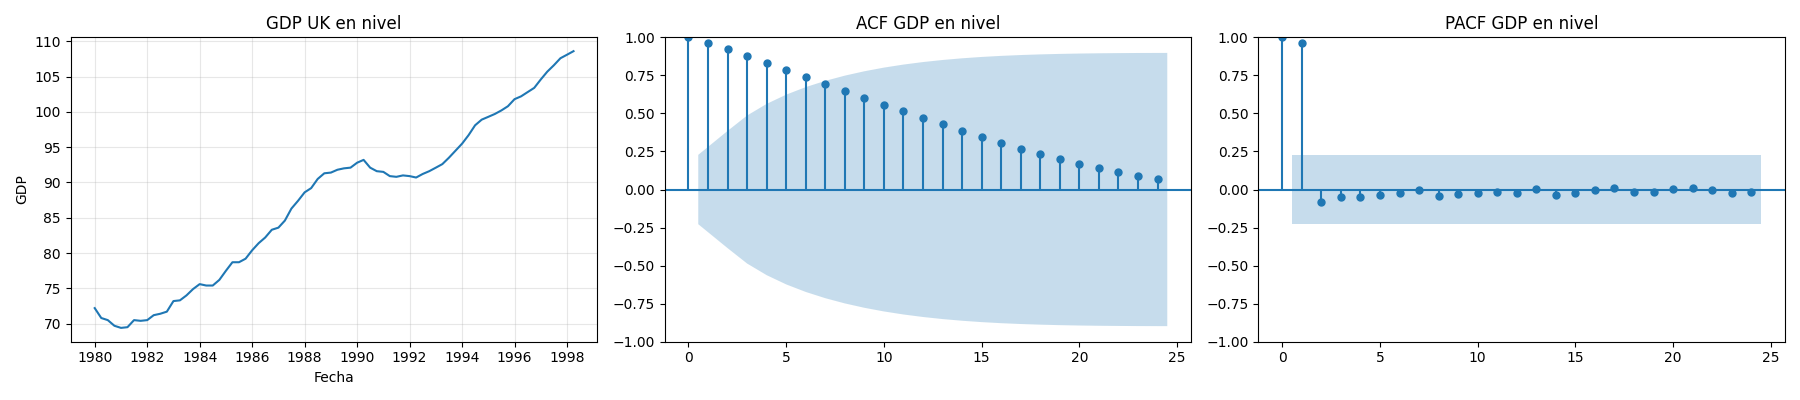
\includegraphics[width=0.95\textwidth]{grafico_1_GDP_ACF_PACF.png}
\caption{GDP en nivel: serie, ACF y PACF}
\end{figure}

Al tomar la primera diferencia logarítmica, la serie cambia de comportamiento. La tendencia desaparece y las autocorrelaciones son menores. El ADF rechaza raíz unitaria con p-value 0.0023, por lo que el GDP se trata como una serie integrada de orden uno.

\begin{figure}[H]
\centering
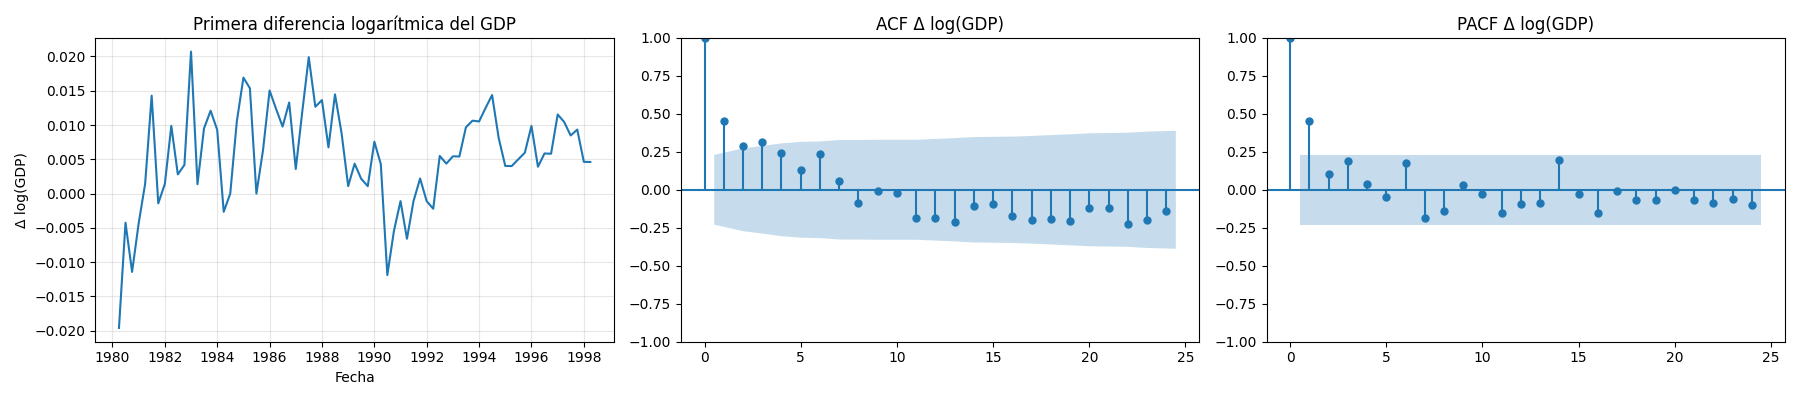
\includegraphics[width=0.95\textwidth]{grafico_2_Direfencia_Log_ACF_PACF.png}
\caption{Primera diferencia logarítmica del GDP: serie, ACF y PACF}
\end{figure}

\begin{table}[H]
\centering
\caption{Test ADF para GDP}
\begin{tabular}{lrrc}
\toprule
Serie & ADF stat & p-value & Rechaza RU 5\% \\
\midrule
GDP nivel & -0.6381 & 0.8621 & No \\
$\Delta\log(GDP)$ & -3.8676 & 0.0023 & Sí \\
\bottomrule
\end{tabular}
\end{table}

\subsection{Selección de modelos ARIMA}

Como la serie es $I(1)$, se estimaron modelos ARIMA$(p,1,q)$. Se compararon cuatro candidatos. El ARIMA(1,1,1) obtiene el menor AIC y el menor BIC. Además, su Durbin-Watson es 2.0677, cercano a 2, lo que es consistente con baja autocorrelación residual.

\begin{table}[H]
\centering
\caption{Comparación de modelos ARIMA candidatos}
\begin{tabular}{lrrrr}
\toprule
Modelo & AIC & BIC & Log-Likelihood & Durbin-Watson \\
\midrule
ARIMA(1,1,1) & -527.4905 & -520.6191 & 266.7453 & 2.0677 \\
ARIMA(1,1,0) & -522.6666 & -518.0857 & 263.3333 & 2.1871 \\
ARIMA(2,1,1) & -519.3491 & -510.1873 & 263.6746 & 2.1896 \\
ARIMA(0,1,1) & -504.4093 & -499.8284 & 254.2046 & 1.4687 \\
\bottomrule
\end{tabular}
\end{table}

La significancia de parámetros también favorece al ARIMA(1,1,1). El componente AR(1) es significativo y el MA(1) también. En cambio, en ARIMA(2,1,1) los parámetros principales no son significativos, por lo que el mayor número de parámetros no parece justificado.

\begin{table}[H]
\centering
\caption{Significancia de parámetros ARIMA}
\begin{tabular}{llrrc}
\toprule
Modelo & Parámetro & Coeficiente & p-value & Sig. 5\% \\
\midrule
ARIMA(1,1,0) & ar.L1 & 0.6793 & 0.0000 & Sí \\
ARIMA(0,1,1) & ma.L1 & 0.5172 & 0.0000 & Sí \\
ARIMA(1,1,1) & ar.L1 & 0.8739 & 0.0000 & Sí \\
ARIMA(1,1,1) & ma.L1 & -0.3565 & 0.0183 & Sí \\
ARIMA(2,1,1) & ar.L1 & 0.2593 & 0.8201 & No \\
ARIMA(2,1,1) & ar.L2 & 0.3488 & 0.6576 & No \\
ARIMA(2,1,1) & ma.L1 & 0.3934 & 0.7372 & No \\
\bottomrule
\end{tabular}
\end{table}

\subsection{Diagnóstico de residuos}

Después de seleccionar ARIMA(1,1,1), se revisaron los residuos. La ACF y PACF residual no muestran autocorrelaciones relevantes fuera de las bandas. El test de Ljung-Box tampoco rechaza autocorrelación residual en los rezagos evaluados.

\begin{figure}[H]
\centering
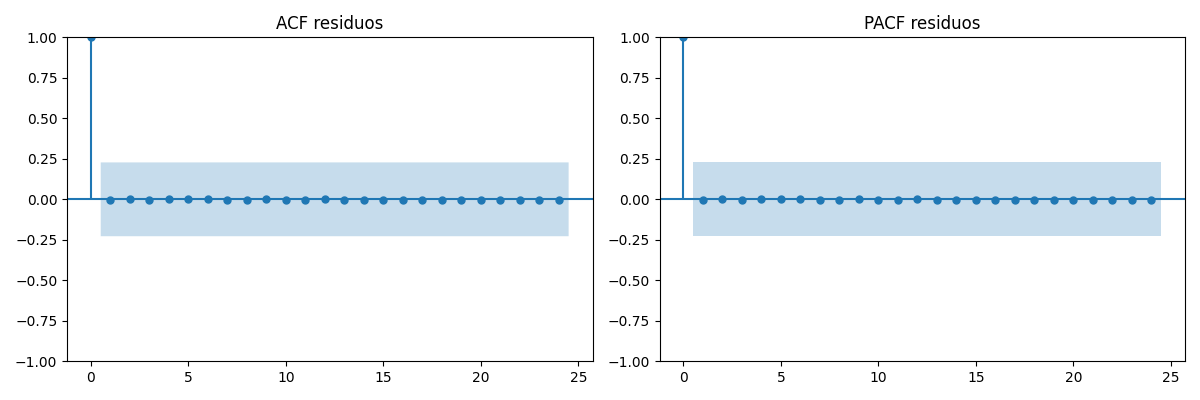
\includegraphics[width=0.85\textwidth]{grafico_4_Dicgnostico_de_Residuos.png}
\caption{Diagnóstico de residuos del modelo ARIMA(1,1,1)}
\end{figure}

\begin{table}[H]
\centering
\caption{Test Ljung-Box sobre residuos}
\begin{tabular}{lrr}
\toprule
Rezago & LB Statistic & p-value \\
\midrule
4 & 0.0025 & 1.0000 \\
8 & 0.0043 & 1.0000 \\
12 & 0.0057 & 1.0000 \\
\bottomrule
\end{tabular}
\end{table}

Con esto, el modelo seleccionado cumple razonablemente con el diagnóstico Box-Jenkins dentro de muestra. La serie fue diferenciada para lograr estacionariedad, se estimaron candidatos, se eligió por criterios de información y se revisaron residuos.

\subsection{Comentario sobre pronóstico}

El ajuste dentro de muestra no debe confundirse con un ejercicio predictivo completo. Para proyectar GDP hacia adelante, el modelo tendría que evaluarse fuera de muestra o con un esquema de validación temporal. Además, la muestra termina en 1998, por lo que pronosticar hasta 2022-2030 exigiría asumir estabilidad de parámetros por un período demasiado largo. Ese supuesto no es inocente en una serie macroeconómica.

\subsection{Conclusión de Metodología Box-Jenkins}

El GDP se comporta como una serie $I(1)$. Una vez tomada la primera diferencia logarítmica, el modelo ARIMA(1,1,1) captura adecuadamente la dependencia temporal observada. El modelo no garantiza buen pronóstico futuro por sí solo, pero sí es una especificación defendible para el análisis solicitado.

\newpage
\section{Conclusión final}

El trabajo deja tres resultados principales. Primero, la estacionariedad no es un trámite previo: cuando se ignora, la inferencia puede mostrar relaciones que no existen. Segundo, la evidencia dentro de muestra debe tomarse con cautela, porque puede desaparecer al evaluar fuera de muestra. Tercero, una señal estadística no siempre se transforma en una decisión económica útil.

La Parte 1 mostró el riesgo de regresión espuria. La Parte 2 mostró que la predictibilidad con \textit{commodity currencies} aparece en algunos casos, pero no de forma robusta al cambiar el criterio de evaluación. La Parte 3 mostró cómo aplicar Box-Jenkins de manera ordenada para identificar, estimar y diagnosticar un modelo ARIMA.

En conjunto, la conclusión es moderada: hay señales predictivas en ejercicios específicos, pero no son lo suficientemente estables como para afirmar una capacidad predictiva general. En finanzas, comparar contra benchmarks simples y evaluar fuera de muestra termina siendo tan importante como obtener un buen ajuste dentro de muestra.

\end{document}
